\documentclass[12pt]{article}

\usepackage[T1]{fontenc}
\usepackage{lmodern}
\usepackage{titling}
\usepackage{graphicx}
\graphicspath{{./images/}}
\usepackage{subcaption}
\usepackage[none]{hyphenat}
\usepackage{mathtools}
\usepackage{hyperref}
\usepackage[shortlabels]{enumitem}
\usepackage{float}
\usepackage{microtype}
\usepackage{tikz}
\newcommand*\circled[1]{\tikz[baseline=(char.base)]{
		\node[shape=circle,draw,inner sep=0pt] (char) {#1};}}

\usepackage
[
a4paper,% other options: a3paper, a5paper, etc
left=2cm,
right=2cm,
top=4cm,
bottom=4cm,
% use vmargin=2cm to make vertical margins equal to 2cm.
% us  hmargin=3cm to make horizontal margins equal to 3cm.
% use margin=3cm to make all margins  equal to 3cm.
]
{geometry}
\setlength{\droptitle}{-10em}

\title{Coursework 3 --- LAST ONE WOHOOO!}
\author{Dobrik Georgiev \\ \small dgg30@cam.ac.uk}

\begin{document}

\maketitle
~\\
\textit{\circled{1.} Describe static and dynamic flow analysis of mobile data
inside a device.}

\begin{itemize}
    \item Static analysis --- The static analysis approach tries to cover
        all possible execution paths of the program. The complete code is
        statically analyzed without need of its execution, then
        the control flow graph (CFG) of program is created. The CFG is
        used to trace the flow of sensitive information from sources
        to sinks. Modern static analyzers convert programs code into some
        intermediate representations, which can be effectively processed to
        generate CFGs. Static analysis takes more time to analyze the program
        than dynamic analysis as it processes the complete code and all
        execution paths. However, it has no realtime performance overhead,
        as processing is done statically before the code is actually
        executed.
        \begin{figure}[H]
            \centering
            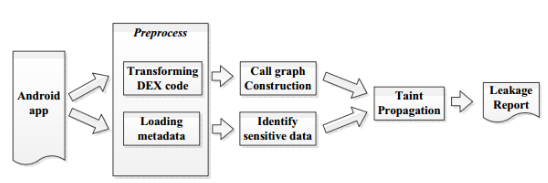
\includegraphics[width=300pt]{LeakMiner.png}
        \end{figure}
        In the figure above the architecture of one static analysis tool --
        LeakMiner is given. E.g. Android applications are executed in Dalvik
        bytecode, therefore this tool first converts  bytecode back to Java
        code and extracts the metadata of the application, such as permissions,
        to help identify sensitive data. Using this Meta data, the system then
        filters relevant API calls. The data flow analysis technique is used to
        form control flow graph of all instructions and data points dependent
        on these API calls. If these data points are propagated over the
        network or logged, a leak path is identified and reported.
    \item Dynamic analysis --- Dynamic analysis monitors the behaviour of
        applications to identify privacy leaks as they are executed. In dynamic
        analysis, the focus is on how the program or application performs on
        a sensitive input data. By performing DFA through the system, users can
        be warned about any potential privacy leak through their devices.
        However, dynamic analysis tools require the actual device or emulator
        to perform the analysis. Moreover, these tools also have performance
        overheads as real time analysis of the application is performed.
        \begin{figure}[H]
            \centering
            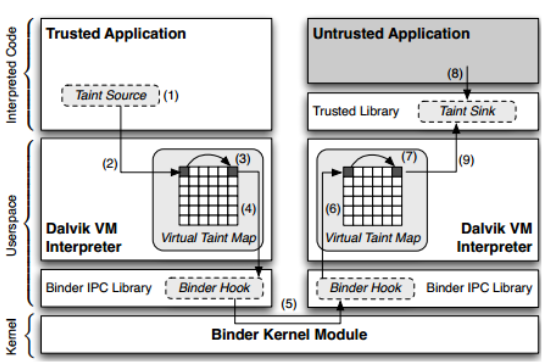
\includegraphics[width=300pt]{TaintDroid.png}
        \end{figure}
        The figure above shows the architecture of TaintDroid, a dynamic
        tool to detect inter application data flow privacy leaks. Information
        is tainted (1) in the trust application. The taint interface
        stores specified tag markings in a virtual taint map and also
        interfaces (2) with Dalvik Vm. The Dalvik VM propagates (3)
        taint tags as applications use the information included. When
        a trusted application uses a modified IPC library (4), taint
        tags are included in the parcel with information and is
        transferred (5) through kernel transparently to untrustworthy
        application. At receiving end, the modified IPC library removes taint
        tags from the parcel and assigns(6) it to all values using the map and
        Dalvik VM propagates (7) these tags to the application. When an
        untrustworthy application invokes taint sink library (8), it
        retrieves tags from the data and reports the event (9).
\end{itemize}

A (not so) quick note on DFA: Data Flow Analysis (DFA) technique is very popular
to track the flow of sensitive information. This technique  is  dependent  on
the  source  and  sink  of  the  data. On  a  higher  level,  this  technique
looks  for  routes  between data  sources  and  sinks  in  mobile  OSs  as
applications  run within  them.  Data  sources  are  sources  of  sensitive
data  such as  location,  file,  database  and  contacts.  While  data  sinks
are points  that  can  leak  out  or  leave  the  mobile  device  such  as the
internet or any other mechanism that transmits data out of the system. Any flow
of data from source to sink without the user's consent can be classified as
privacy leakage.
~\\
~\\
\textit{\circled{2.} Illustrate Mobile Sensing Privacy issues.}

Sensors could release a lot of information, if interpreted wisely --- different
users can use the same device in a different way, so (e.g.) accelerometer
+ touch screen patterns could be enough to give out user identity. Even with
a large anonymized datasets, there would be enough correlated to identify
a single user, just by profiling activity and patterns, such as always going to
the gym after work or that user A and user B always stick together.
\\
\\
\textit{\circled{3.} Mobility prediction -- discuss how a user has only a few
significant places and these can be used together with temporal features for
mobility prediction.}

First the significant places need to be extracted --- there are plenty of
possibilities for doing that, but two of them are:
\begin{itemize}
    \item Extracting Places from GPS Data --- apply a 2D Gaussian distribution
        weighted by the residence time at each GPS point. This means that at
        each point the Gaussian distribution uniformly contributes also to
        nearby points, smoothing out values that are close together.  The
        value of  the  variance  for  the  Gaussian  distributions  can
        correspond to the GPS accuracy.  The resulting frequency map contains
        peaks which give information about the position of popular locations:
        regions that are above a certain threshold are considered as
        significant places. The threshold can be chosen as a fraction of the
        maximum value of the frequency map.
    \item Extracting  Places  from  WiFi  Logs --- Alternatively,  we  can
        derive  significant  places from user registrations to 802.11 access
        points. Since these access points are fixed and easily identifiable from
        their globally unique MAC address, this information can be exploited
        to extract visit patterns to a set of locations in a straightforward
        manner. From this point of view, the most frequently seen access points
        are natural candidates to represent significant places. Hence, we can
        define as popular places for a user the access points he/she connects to
        more often, providing that a sufficient number of visits \textit{n} has been
        recorded to a given access point.
\end{itemize}

Now for predicting the behaviour: The history of visits of a user to each of
its significant locations is considered. Then, for each location we try to
predict when the next visits will take place and for how long they will last.
After this estimation, the predictions obtained for different locations is
analyzed, in order to produce a unique prediction of where the user will be at
a given future instant of time. 

\textit{(Skipping the gore details of the maths, email me if its needed to add it.)}

For example, if the last three visits of a certain user to a location are Monday
at 6:30pm, Monday at 10:00pm and Tuesday at 8:15am, we analyze the history of
visits in order to find sequences that are numerically close to (6:30pm,
10:00pm, 8:15am), e.g. (6:10pm, 9:50pm, 8:35am) and (6:35pm, 10:10pm, 8:00am).
Then, assuming that the next visits that follow these subsequences start at
1:10pm and 12:40pm and last for 40 and 30 minutes respectively, we estimate the
next visit at 12:55pm for 35 minutes, averaging both arrival times and duration
times.
\\
\\
\textit{\circled{4.} For the mesh architecture discussed in lectures, explain
why the complex routing protocols designed for mesh networks were not used.}

(\textbf{Truly} no idea, just writing the first thing that came to my mind and
seems logical.)

Each of the mesh networks could be for a different application, e.g. one for
turning lights at the same time, another for tuning temperature at different
rooms, etc. Each application would benefit more from a different ad-hoc routing
protocol. Moreover, similar applications could be used on a different scale,
e.g. one used over the whole area of a big house, another used always in
a single room. Clearly one and the same protocol won't do well for all cases.
\\
\\
\textit{\circled{5.} When in a connection, two BLE devices use frequency
hopping to communicate reliably. When advertising, a BLE device sends the
advertising packet on each of three dedicated channels in turn.}

I am really bad at the BLE stuff, bear that in mind when checking the question.
\begin{enumerate}[1.]
    \item \textit{Explain at a high level what frequency hopping
        is and how it provides resilience to interference from both BLE and
        non-BLE sources.}

        Adaptive Frequency Hopping (AFH) is available for the BLE connection
        state only. The term adaptive is used to indicate, that during the
        hopping process channel conditions are permanently monitored to
        identify occupied or low quality channels, which are stated bad
        channels. The bad channels are excluded from the available channels
        within the hopping pattern until they become good channels again.

        Bad channels are also remapped to good ones, e.g. if there is interference with
        wi-fi channels.
    \item \textit{Why does advertising not use frequency hopping?}
        As far as I am aware for communication with frequency hopping you need
        to have the clocks of the two devices synchronised as the hopping
        pattern is unique and derived from master clock. (Saw that here:
        \url{https://scdn.rohde-schwarz.com/ur/pws/dl_downloads/dl_application/application_notes/1c108/1C108_0e_Bluetooth_BR_EDR_AFH.pdf})

        Also, if we were advertising and hopping that would take a lot of time
        to discover a connection.
    \item \textit{Explain why there are three advertising channels
        (rather than two or four, etc) and why they are where they are in the
        radio band.}

        Reduces time to find devices. Not sure why there are there and why they
        are 3. (Apart from the fact, that if we had 10 advertising is slower.)
        \url{https://www.argenox.com/library/bluetooth-low-energy/ble-advertising-primer/}
        mentions that there could be more than $3$ in the latest BL specs, but
        $3$ is the common case.
\end{enumerate}

\textit{\circled{6.} What is a Voronoi tessellation and how is it useful?}

Partitioning of a plane into regions based on distances to points in a specific
subset of the plane. A set of points is specified beforehand, and for each seed
there is a corresponding region consisting of all points closer to that seed
than to any other. These regions are called Voronoi cells and the way they 
break up the space is called Voronoi tessellation.

It is useful as the Voronoi tessellation (in particular the Centroidal Voronoi
Tesselation, CVT) can optimally distribute robots, so that the average distance
between robots and all robots in all points in their repsective cells is
minimised. (CVT is when points have 'masses'; 'masses' can be thought of as
importance)
\\
\\
\textit{\circled{7.} How does Lloyd's algorithm work?}

\textit{Aside node: LLoyd's is actually used for k-means clustering (afaik). This here
is LLoyd's algorithm applied to Voronoi tessellation.}

\begin{enumerate}
    \item Construct the Voronoi partition for the generators.
    \item Compute the centroids of these regions by a classic Voronoi
        tessellation.
    \item  Move generators to centroids.
    \item Repeat until convergence.
\end{enumerate}

\textit{Yet another aside: In the k-means clustering, LLoyd's can converge to
a local minimum, but here always converges to a CVT.}
\\
\\
\textit{\circled{8.} What is the difference between a centralised and
decentralised multi-robot system?}

Exactly what it says on the tin --- in centralised multi-robot system there is
one control unit (e.g. as the base station with the bats last supervision) with
all robots communicating with it and receiving commands from there/returning
data to there. Decentralised system is exactly the opposite -- it has no `base
station', communication happens between robots and messages propagate
eventually through the `swarm', robots decide their actions on their own (or at
most with those around it), etc.

In terms of which is better --- depends on application. Centralised is more
optimal wrt to decentralised, but it's also prone to failure (just break the
control unit or prohibit it's communication) plus it requires some sort of
synchronisation. Decentralised is sub-optimal, the algorithms applied there
will eventually converge to optimal (but this time can be the infinity), but
it's more robust, in the sense that one failing robot may not cause a lot of
disruption.
\\
\\
\textit{\circled{9.} Name two ways of estimating the state of a robot (e.g.,
position). What are potential pitfalls of using such algorithms in
a multi-robot system?}

Collaborative Localisation using some filter, e.g. (E)KF or particle.

Some sort of consensus algorithm. (There isn't any particular second algorithm
in the lectures.)

A pitfalls I can think of is that with such `decentralised' algorithms you can 
have contradicting views (i.e. half of the robot think pt. A is south, another
half think it's north).

Yet another disadvantage is that global tasks are difficult to achieve and
require more complex algorithms (e.g. imagine making all of the robot move
southeast in a wiggly manner, without colliding at each other).

Also, malicious (or just totally failed) nodes can be a pain --- they can
fool the other robots into wrong assumptions about the environment or into
taking wrong actions (e.g. moving in a different direction).

\end{document}
